\section{Teddy Gideon Manik(1174038)}

\subsection{Koordinat}
\par
Koordinat adalah sistem koordinat yang memungkinkan setiap lokasi di Bumi ditentukan oleh serangkaian angka, huruf, atau simbol. Koordinat sering dipilih sedemikian sehingga salah satu angka mewakili posisi vertikal dan dua atau tiga angka mewakili posisi horisontal; sebagai alternatif, posisi geografis dapat diekspresikan dalam vektor Kartesius tiga dimensi. Pilihan umum koordinat adalah lintang, bujur dan ketinggian. Untuk menentukan lokasi di pesawat membutuhkan proyeksi peta. secara singkanya yaitu salah satu dari dua garis lintang dan bujur yang persimpangannya menentukan titik geografis suatu tempat.
Dalam geometri, sistem koordinat adalah suatu sistem yang menggunakan satu atau lebih bilangan, atau koordinat, untuk secara unik menentukan posisi suatu titik atau unsur geometris lain pada manifold seperti ruang Euklides. Urutan koordinat adalah signifikan, dan mereka kadang-kadang diidentifikasi oleh posisi mereka dalam tuple dan kadang-kadang dengan huruf, seperti dalam "x-coordinate". Koordinat diambil untuk menjadi bilangan real dalam matematika dasar, tetapi mungkin bilangan kompleks atau elemen-elemen dari sistem yang lebih abstrak seperti sebuah cincin komutatif. Penggunaan sistem koordinat memungkinkan masalah dalam geometri untuk diterjemahkan ke dalam masalah-masalah tentang angka dan sebaliknya; ini adalah dasar dari geometri analitis.[3]


\begin{figure}[H]
	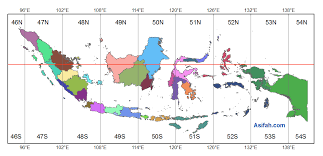
\includegraphics[width=4cm]{figures/1174038/peta koordinat indonesia.png}
	\centering
	\caption{Koordinat Indonesia}
\end{figure}

\subsection{Link}
\href{https://https://youtu.be/gIAfrXKGDCI}{LINK Youtub, JANGAN LUPA SASKREB}
\subsection{Plagiarism}
\begin{figure}[H]
	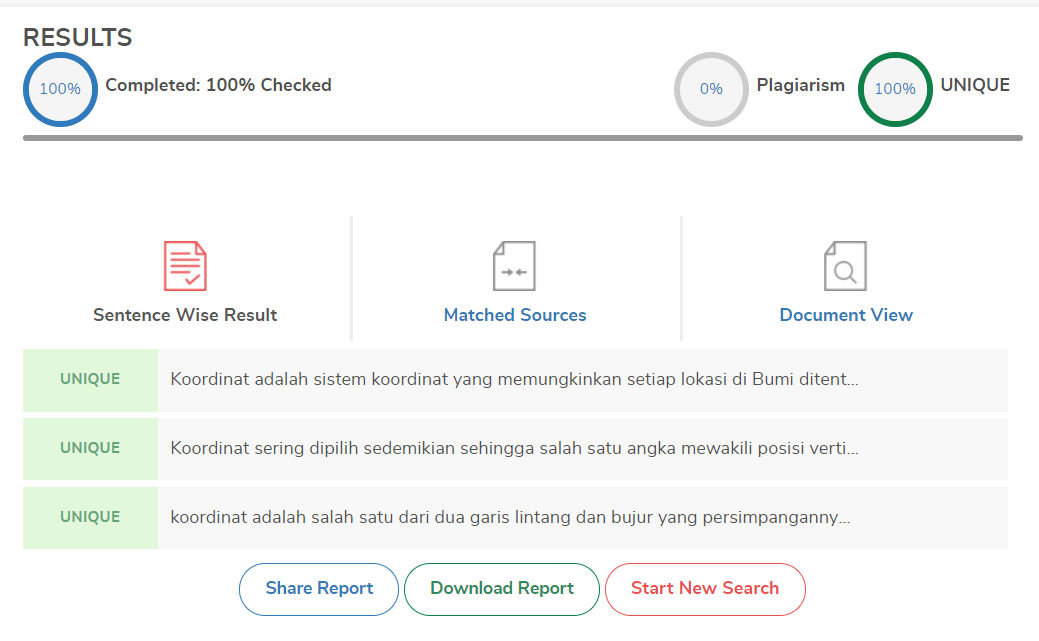
\includegraphics[width=4cm]{figures/1174038/plagiarism.png}
	\centering
	\caption{Plagiarism}
\end{figure}